\lstinputlisting[language=bash,basicstyle=\small]{python_codes/fieldstone_02/keywords}

\begin{center}
Code at \url{https://github.com/cedrict/fieldstone/tree/master/python_codes/fieldstone_02}
\end{center}

\par\noindent\rule{\textwidth}{0.4pt}
%%%%%%%%%%%%%%%%%%%%%%%%%%%%%%%%%%%%%%%%%%%%%%%%%%%%%%%%%%%%%%%%%%%%%%%%%%%%%%%%%%%%%%%%%

This stone carries out the benchmark of Section~\ref{ss:stokes_sphere2D}
with $Q_1\times P_0$ elements using the penalty formulation.
The domain is a unit square and the fluid is characterised 
by $\rho=1$ and $\eta=1$ 
while the sphere is characterised 
by $\rho=1.01$ and $\eta=1000$.
The gravity vector is $\vec{g}=(0,-1)$. 
Boundary conditions are free slip (FS) on all sides, no slip on all sides (NS)
or free slip on the sides and bottom and open on top (OT).
Viscosity and density directly computed at the quadrature points.
The results are presented in Section~\ref{ss:stokes_sphere2D}.

\begin{center}
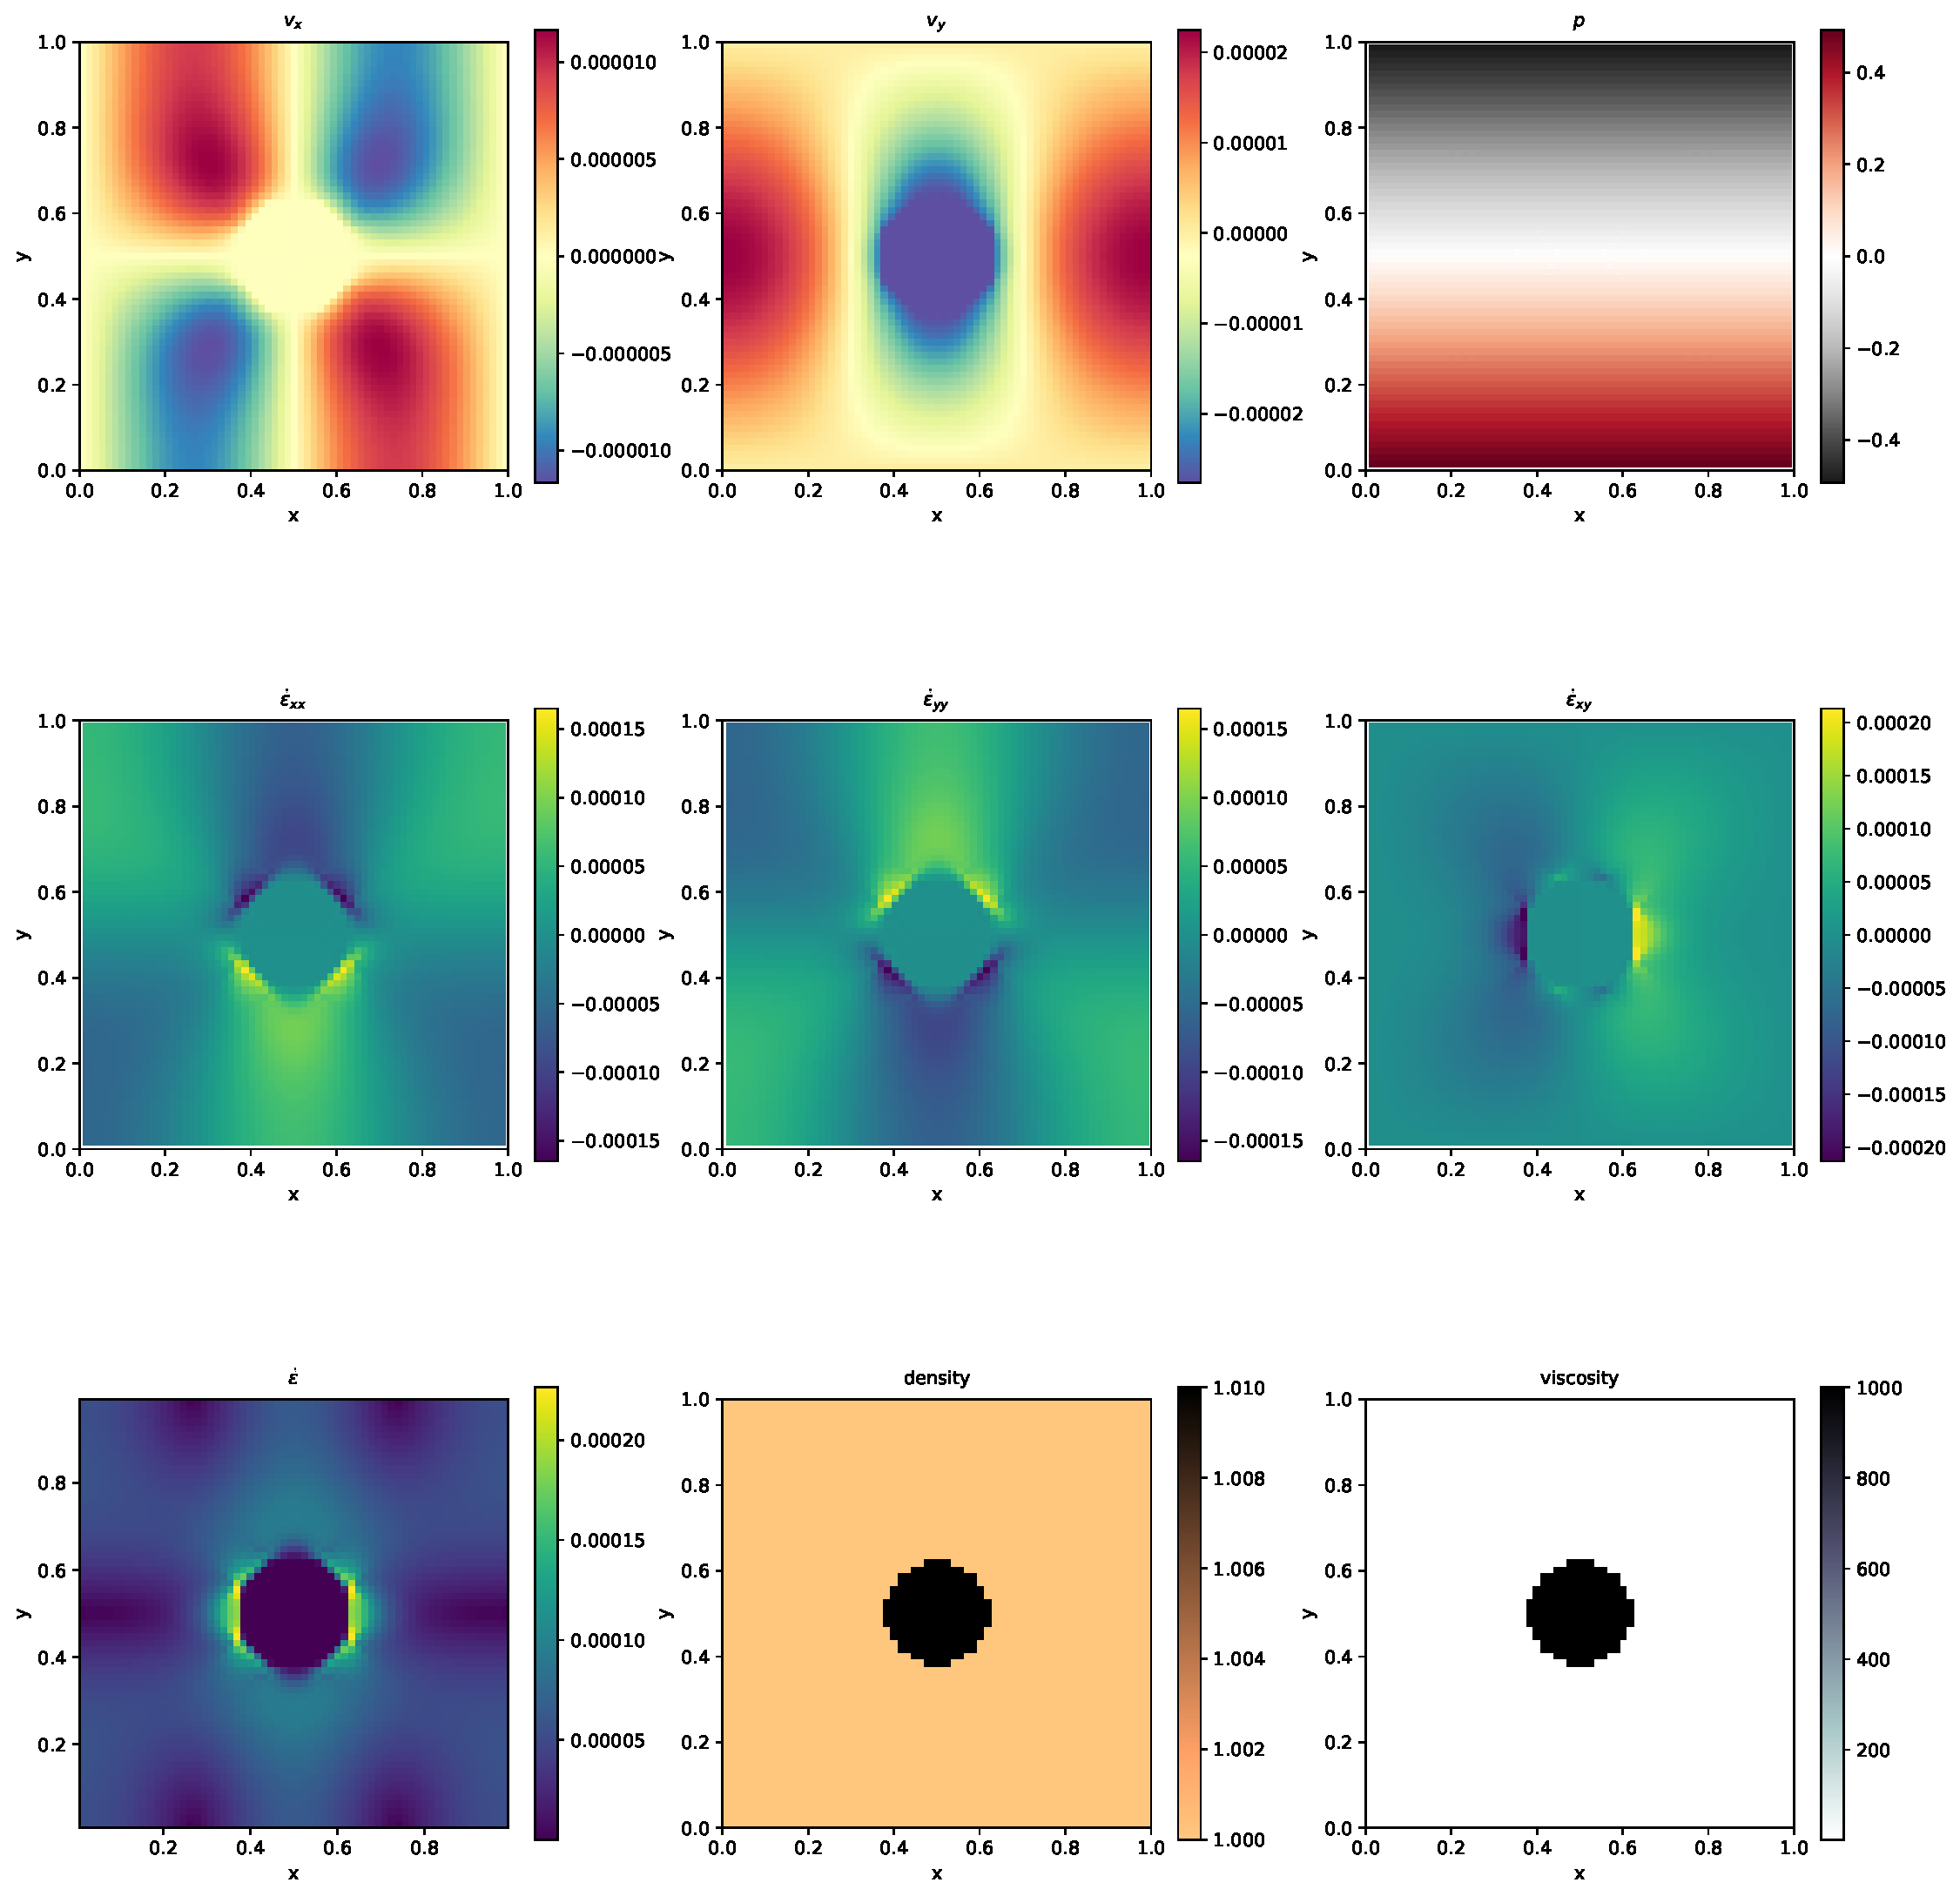
\includegraphics[width=15cm]{python_codes/fieldstone_02/solution64FS.pdf}\\
{\captionfont Results on a 64x64 grid with FS boundary conditions.}
\end{center}


